%% =====================================================================
%% PACER: A Perturbation-Aware Contrastive Framework for Long-Tail
%%        Multimodal Recommendation --- KSE 2026 (v34, camera-ready)
%% Authors: Minh-Khoi Le(corresponding)
%% VNU University of Engineering and Technology, Hanoi, Vietnam
%% =====================================================================
\documentclass[conference]{IEEEtran}
\IEEEoverridecommandlockouts

% ===================== Encoding =====================
\usepackage[utf8]{inputenc}
\usepackage[T1]{fontenc}
\usepackage[english]{babel}
\DeclareFontShape{T1}{ptm}{m}{scit}{<->ssub*ptm/m/it}{}

% ===================== Math =====================
\usepackage{amsmath,amssymb,amsfonts,amsthm}
\usepackage{mathtools}
\usepackage{bm}

% ===================== Graphics & Diagrams =====================
\usepackage{graphicx}
\usepackage{tikz}
\usepackage{pgfplots}
\pgfplotsset{compat=1.18}
\usepgfplotslibrary{groupplots}
\usetikzlibrary{
  arrows.meta, calc, positioning, shapes.geometric, shapes.misc,
  fit, backgrounds, decorations.pathreplacing, decorations.markings,
  patterns, matrix, chains, scopes
}

% ===================== Tables & Misc =====================
\usepackage{booktabs}
\usepackage{multirow}
\usepackage{array}
\usepackage{enumitem}
\usepackage{xcolor}
\usepackage{cite}
\usepackage{xspace}
\usepackage{microtype}

% ===================== Colours for diagrams =====================
\definecolor{accentteal}{HTML}{20808D}
\definecolor{accentdark}{HTML}{1B474D}
\definecolor{accentterra}{HTML}{A84B2F}
\definecolor{accentgold}{HTML}{D19900}
\definecolor{accentcyan}{HTML}{BCE2E7}
\definecolor{accentolive}{HTML}{848456}
\definecolor{accentmauve}{HTML}{944454}
\definecolor{bgsoft}{HTML}{F7F6F2}
\definecolor{passgreen}{HTML}{437A22}
\definecolor{negativered}{HTML}{A13544}
\definecolor{accentblue}{HTML}{006494}

% ===================== Shortcuts =====================
\newcommand{\Lcal}{\mathcal{L}}
\newcommand{\Ucal}{\mathcal{U}}
\newcommand{\Ical}{\mathcal{I}}
\newcommand{\Ecal}{\mathcal{E}}
\newcommand{\norm}[1]{\left\lVert #1 \right\rVert}
\newcommand{\dvr}{DVR\xspace}

% ===================== Metadata =====================
\title{PACER: A Perturbation-Aware Contrastive Framework\\for Long-Tail Multimodal Recommendation}

\author{
\IEEEauthorblockN{Minh-Khoi Le$^{*}$}
\IEEEauthorblockA{VNU University of Engineering and Technology, Hanoi, Vietnam\\
khoilm@vnu.edu.vn}
\thanks{$^{*}$Corresponding author.}
}

\begin{document}
\maketitle

% =====================================================================
\begin{abstract}
Multimodal recommenders regularise graph propagation with an InfoNCE
contrastive head, yet the frozen ResNet-50 and Sentence-BERT features
they consume carry sensor and semantic noise that content-graph
propagation compounds---penalising long-tail items, whose small
neighbourhoods average that noise away least effectively. We propose
\textbf{PACER} (Perturbation-Aware Contrastive Encoder
Regularisation), whose central finding is
\emph{distributional}: a lightweight two-view denoiser ---
\textbf{\dvr} (Dual-View Reweighting) --- reallocates capacity from
Head to Mid/Tail at nearly constant overall Recall@20. \dvr learns semantic-aware (SAV) and interest-aware (IAV)
views, fuses them by a complement-weighted consensus, and pulls the
trunk toward the denoised view via InfoNCE. In a matched A0-vs.-A1
ablation that toggles \dvr alone, Mid- and Tail-tercile Recall@20 rise
by $+6.1\%$/$+12.1\%$ on Amazon Clothing and $+38.1\%$/$+65.3\%$ on
Amazon Sports ($d_z{=}4.32/5.52$, $p{<}10^{-3}$), with Head
statistically flat on both and overall Recall@20 nearly unchanged.
Against a capacity-matched MMHCL baseline --- the same code with the
embedding width raised to PACER's $d{=}320$ --- PACER gains
$+10.48\%$ Recall@20 and $+13.07\%$ NDCG@20 on Clothing
($+7.04\%$/$+8.56\%$ on Sports); the larger gains against MMHCL's
native $d{=}64$ setting ($+18.92\%$/$+21.17\%$) are substantially
attributable to embedding capacity alone. All of this costs only
$d{+}2$ extra parameters ($322$ at $d{=}320$).
\end{abstract}

\begin{IEEEkeywords}
Multimodal recommendation, graph contrastive learning, view perturbation,
noise-robust item modeling, long-tail recommendation.
\end{IEEEkeywords}

% =====================================================================
\section{Introduction}
% =====================================================================

Multimodal recommender systems fuse image, text, and interaction
signals over the user--item graph, and now form the backbone of
e-commerce, streaming, and short-video platforms
\cite{guo2025mmhcl,li2026multiview,hao2026itcohd}. Recent work has
pushed representation quality with hypergraph propagation
\cite{guo2025mmhcl,hao2026itcohd}, spectrum-based fusion
\cite{ong2025spectrum,wang2026damps}, dual-path modality routing
\cite{yan2025compensating}, interest-tree augmentation of the modality
graph \cite{meng2025tamer}, noise-robust item modelling with dynamic
multi-view contrastive learning \cite{gong2026noise}, and multi-level
self-supervision \cite{xu2025mentor}. Regardless of fusion strategy,
however, the training signal that ties everything together is almost
invariably the InfoNCE contrastive loss.

The failure mode we target is upstream of the loss: the frozen
encoders are noisy, and propagation amplifies rather than attenuates
that noise. Background clutter in images and boilerplate in product
titles enter as sensor and semantic noise; content-graph
propagation then compounds them across layers before content is
fused with the collaborative representation. Long-tail items are the
primary casualties: their neighbourhoods are small, so the
neighbourhood averaging that graph propagation relies on cannot smooth
out the noise, and the InfoNCE head then absorbs the resulting
representation drift into its logits. By \emph{perturbation} we mean
exactly this propagated multimodal noise, not an adversarial attack.

This long-tail harm is not only a technical pathology but the research
target. Long-tail items form the bulk of the catalogue yet receive
little exposure; improving Mid/Tail retrieval raises coverage,
diversity, and long-run marketplace revenue. Aggregate top-$K$
metrics, which current multimodal papers predominantly report, can
mask the fact that gains accrue mainly to the Head---precisely the
gap that our Head/Mid/Tail tercile evaluation is designed to expose.

\smallskip
\noindent\textbf{Our contributions.}
\begin{itemize}[leftmargin=1.2em,itemsep=2pt,topsep=3pt,parsep=0pt]
  \item \emph{Distributional finding.} On two Amazon catalogues,
        adding a $d{+}2$-parameter two-view denoiser to an
        MMHCL-style trunk reallocates representational capacity from
        Head to Mid/Tail at nearly constant overall Recall@20. In the
        matched A0-vs.-A1 pipeline (same width, depth, and schedule)
        \dvr adds $+6.1\%$ Mid and $+12.1\%$ Tail on Clothing and
        $+38.1\%$ Mid and $+65.3\%$ Tail on Sports, with Head flat on
        both; against a capacity-matched MMHCL baseline the
        $250$-epoch cross-model gains are $+24.5\%$ Mid and
        $+20.8\%$ Tail on Clothing ($+45.7\%$/$+46.5\%$ on Sports).
  \item \emph{Parameter-efficient architecture.} The \dvr module
        (Dual-View Reweighting) is a drop-in view-contrastive
        denoiser that composes a semantic-aware view (SAV) and an
        interest-aware view (IAV) and fuses them by
        \emph{subtracting} the softmax-weighted mixture from the raw
        sum (Eq.~\ref{eq:fuse}) --- a complement-weighted consensus
        rule that upweights edges on which both views agree.
        \dvr adapts the two-view design of NRDMC~\cite{gong2026noise} but
        drops its prototype-aware view and its $M$ learnable
        prototypes, costing $d{+}2=322$ extra parameters at the
        reported $d{=}320$ on both datasets.
  \item \emph{Transparent negative-result audit.} A $2{\times}2$
        factorial (Sec.~\ref{sec:factorial}) over an
        RSFPGrowth-blended TAMER-style interest tree and a
        Log$Q$-Laplace popularity debias shows that neither axis
        contributes measurably once \dvr is in place, and the only
        paired contrast reaching $\alpha{=}0.05$ favours
        \emph{disabling} both (B11 vs.\ B00, $p{=}0.040$).
\end{itemize}

\smallskip
\noindent\textbf{Provenance and headline numbers.} PACER reimplements
MACP whitening and the interest-tree item--item
construction following TAMER~\cite{meng2025tamer};
Sec.~\ref{sec:tamerrel} states what we adopt, modify, and drop. On
Amazon Clothing over five fixed seeds,
PACER lifts Recall@20 by $+10.48\%$, NDCG@20 by $+13.07\%$, and
Precision@20 by $+10.28\%$ over a capacity-matched MMHCL reproduction
at the same embedding width (Table~\ref{tab:rq1} also reports the
larger figures against MMHCL's native $d{=}64$ setting). The Sports
replication
(Sec.~\ref{sec:rq5}) reproduces the tercile signature at higher
statistical power.

% =====================================================================
\section{Related Work}
\label{sec:related}
% =====================================================================

\noindent\textbf{Multimodal graph recommenders and noise-robust
modelling.} Modern multimodal recommenders combine collaborative
propagation with modality-specific or fused content-graph branches and
regularise them with contrastive objectives.
MMHCL~\cite{guo2025mmhcl} treats each modality as a hyper-edge;
ITCoHD-MRec~\cite{hao2026itcohd} adds cooperative hypergraph
diffusion; spectrum-based
fusion~\cite{ong2025spectrum,wang2026damps}, multi-view
alignment~\cite{li2026multiview}, dual-path
routing~\cite{yan2025compensating}, MENTOR~\cite{xu2025mentor}, and
self-supervised multimodal GCNs~\cite{kim2024self} vary fusion and
self-supervision schedules but retain vanilla InfoNCE. PACER is
orthogonal: it augments the encoder with a two-view denoising branch
without changing modality fusion or the primary loss family.
Contrastive-SSL foundations~\cite{chen2022intent,liu2021self,liu2023self}
justify InfoNCE-style regularisation; sampled-metric
analysis~\cite{krichene2020sampled} motivates our long-tail tercile
evaluation. NRDMC~\cite{gong2026noise} couples noise-robust item
modelling with dynamic multi-view contrastive learning over three
views (semantic, interest, prototype-aware); \dvr adapts its two-view
design to a parameter-efficient regime, retaining semantic-aware and
interest-aware views with adaptive edge-weight fusion and a view-level
LightGCN, but dropping the prototype-aware view and its $M$ learnable
prototypes $P\in\mathbb{R}^{M\times d}$.

\noindent\textbf{Interest-tree augmentation and popularity debiasing.}
TAMER~\cite{meng2025tamer} redistributes modality features via
a Multi-component Analysis Collaborative Processing (MACP) block
(PCA$\to$ICA and ZCA whitening) and augments the item--item modality
graph with an Interest Tree built by BFS over co-occurrence. PACER
reimplements these steps following TAMER; reported runs use the
PCA$\to$ICA replacement stream (Sec.~\ref{sec:tamerrel});
optionally we source the interest graph from an RSFPGrowth-blended
co-occurrence and wire the augmented similarity into \dvr's
item-side content graph. Log$Q$-corrected softmax is a standard InfoNCE
popularity-bias remedy. Sec.~\ref{sec:factorial} audits both axes
and reports them as neutral/negative once \dvr is present.

\noindent\textbf{Denoising-diffusion recommenders.}
Recent denoising-diffusion
work~\cite{jiang2024diffmm,jiang2024diffkg,nguyen2024diffusion}
addresses noise at the generative layer rather than at the encoder or
the loss; \dvr composes freely with any of these directions.

% =====================================================================
\section{Preliminaries}
\label{sec:prelim}
% =====================================================================

Let $\Ucal$ be the user set, $\Ical$ the item set, and $\mathcal{G} =
(\Ucal \cup \Ical, \Ecal)$ the observed bipartite interaction graph.
Each item $i \in \Ical$ carries a frozen visual feature
$v_i \in \mathbb{R}^{d_v}$ (ResNet-50 pooled), a frozen textual feature
$t_i \in \mathbb{R}^{d_t}$ (Sentence-BERT), and trainable ID embeddings.
The goal is to learn a scoring function $s_\theta(u, i)$ that
maximises Recall@$K$ and NDCG@$K$ on the held-out test set. Following
LightGCN, PACER's collaborative trunk propagates ID ego embeddings over
$L$ layers of
the symmetrically normalised adjacency $\tilde A$:
\begin{equation}
Z^{(\ell+1)} = \tilde A\, Z^{(\ell)},\quad
Z = \tfrac{1}{L+1} \sum_{\ell=0}^{L} Z^{(\ell)}.
\label{eq:lightgcn}
\end{equation}
Standard BPR ranking supplies the primary loss $\Lcal_{\text{BPR}}$;
\dvr (Sec.~\ref{sec:dvr}) contributes an auxiliary
in-batch-negative InfoNCE view loss $\Lcal_{\text{view}}$.

% =====================================================================
\section{The PACER Framework}
\label{sec:pacer}
% =====================================================================

\subsection{Overview}
\label{sec:overview}

\begin{figure*}[t]
\centering
\resizebox{\textwidth}{!}{%
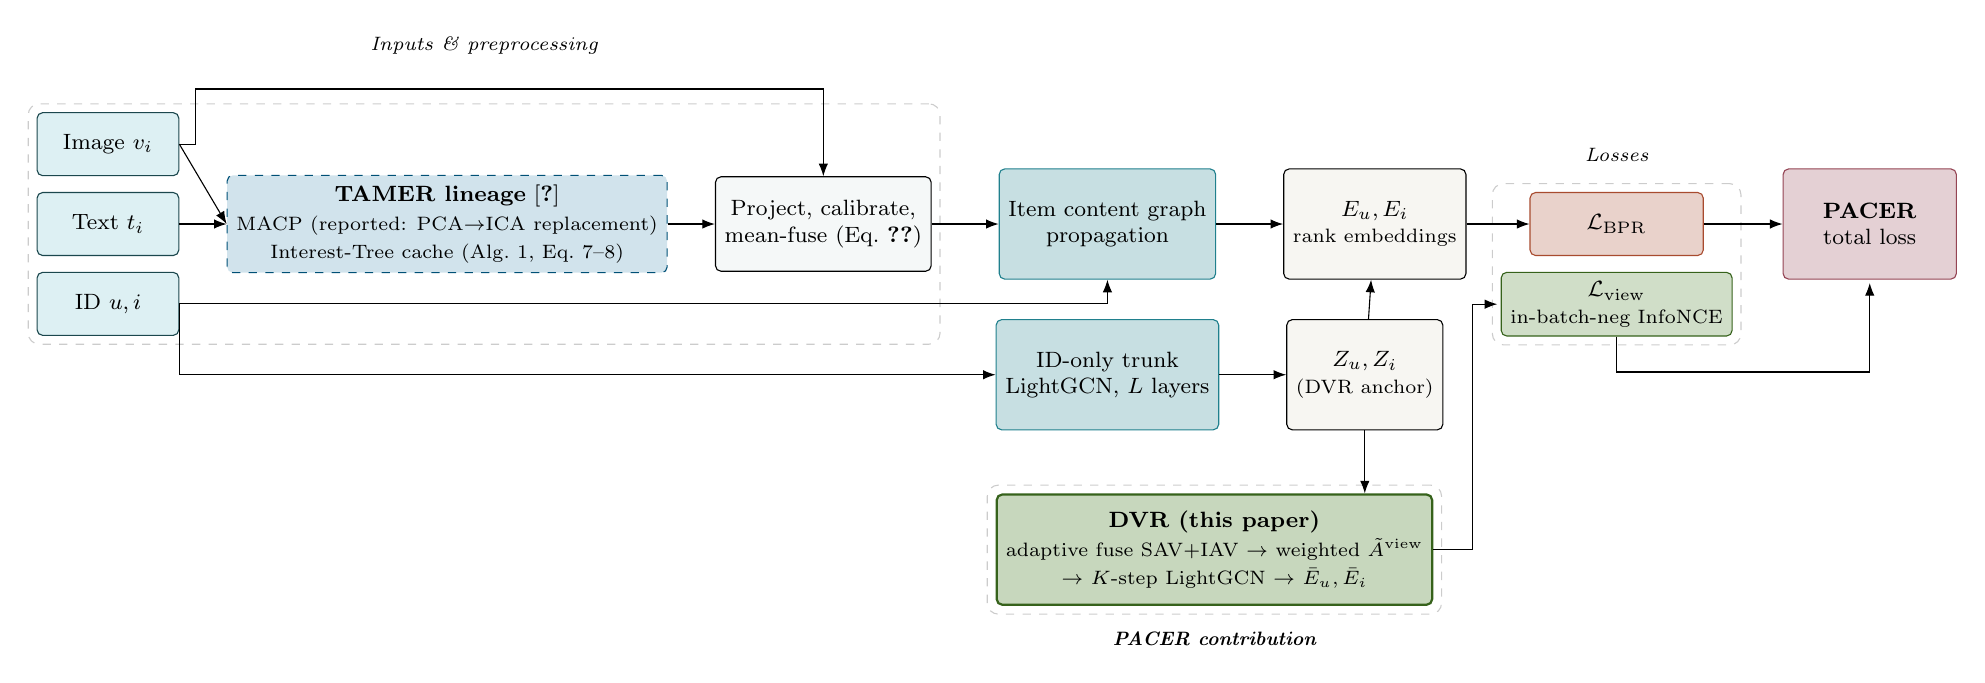
\begin{tikzpicture}[
  font=\footnotesize,
  node distance = 6mm and 8.5mm,
  block/.style={draw, rounded corners=2pt, align=center,
                minimum height=8mm, minimum width=18mm,
                fill=bgsoft, line width=0.4pt},
  modblock/.style={block, fill=accentcyan!50, draw=accentdark},
  gnnblock/.style={block, fill=accentteal!25, draw=accentteal},
  viewblock/.style={block, fill=accentteal!45, draw=accentteal!80!black},
  lossblock/.style={block, fill=accentterra!25, draw=accentterra, minimum width=22mm},
  denblock/.style={block, fill=accentolive!30, draw=accentolive!80!black,
                   minimum width=24mm},
  ctrbblock/.style={block, fill=passgreen!30, draw=passgreen!80!black, thick,
                    minimum width=24mm},
  tamerblock/.style={block, fill=accentblue!18, draw=accentblue!80!black,
                     minimum width=30mm, minimum height=10mm, dashed},
  negblock/.style={block, fill=negativered!12, draw=negativered!60!black, dashed,
                   minimum width=26mm, minimum height=7mm},
  arrow/.style={-{Latex[length=1.6mm]}, line width=0.4pt},
  dasharrow/.style={-{Latex[length=1.6mm]}, dashed, line width=0.4pt, draw=negativered!60!black},
  bgblock/.style={draw=gray!40, dashed, rounded corners=4pt,
                  inner sep=3pt, line width=0.4pt}
]

% ---------------- Inputs ----------------
\node[modblock] (img)  {Image $v_i$};
\node[modblock, below=2mm of img] (txt) {Text $t_i$};
\node[modblock, below=2mm of txt] (id)  {ID $u, i$};

% TAMER-lineage preprocessing (MACP + Interest-Tree cache), audited
\node[tamerblock, right=6mm of txt, align=center] (tamer)
  {\textbf{TAMER lineage}~\cite{meng2025tamer}\\[0.4mm]
   \scriptsize MACP (reported: PCA$\to$ICA replacement)\\[0.2mm]
   \scriptsize Interest-Tree cache (Alg.~1, Eq.~7--8)};

\node[block, right=6mm of tamer, fill=accentcyan!80!black!10, minimum height=12mm]
  (fuse) {Project, calibrate,\\mean-fuse (Eq.~\ref{eq:egofusion})};

% ---------------- Collaborative and content branches ----------------
\node[gnnblock, right=of fuse, minimum width=22mm, minimum height=14mm]
  (hgcn) {Item content graph\\propagation};
\node[gnnblock, below=5mm of hgcn, minimum width=22mm, minimum height=14mm]
  (lgcn) {ID-only trunk\\LightGCN, $L$ layers};

% ---------------- Trunk anchor ----------------
\node[block, right=of lgcn, fill=bgsoft, minimum width=18mm, minimum height=14mm]
  (E) {$Z_u, Z_i$\\\scriptsize (DVR anchor)};
\node[block, right=of hgcn, fill=bgsoft, minimum width=20mm, minimum height=14mm]
  (rank) {$E_u, E_i$\\\scriptsize rank embeddings};

% ---------------- \dvr denoiser (contribution) ----------------
% Left-aligned under the trunk so DVR.east stays left of L_view.west.
\node[ctrbblock, below=8mm of lgcn.south west, anchor=north west,
      minimum width=48mm, minimum height=14mm, align=center] (nrdmc)
  {\textbf{\dvr (this paper)}\\[0.3mm]
   \scriptsize adaptive fuse SAV+IAV $\to$ weighted $\tilde A^{\text{view}}$\\[0.2mm]
   \scriptsize $\to$ $K$-step LightGCN $\to$ $\bar E_u, \bar E_i$};

% ---------------- Losses ----------------
\node[lossblock, right=8mm of rank] (bpr) {$\Lcal_{\mathrm{BPR}}$};
\node[lossblock, below=2mm of bpr, fill=passgreen!25, draw=passgreen!80!black]
  (view) {$\Lcal_{\mathrm{view}}$\\\scriptsize in-batch-neg InfoNCE};

% ---------------- Total ----------------
\node[block, right=10mm of bpr, fill=accentmauve!25, draw=accentmauve,
      minimum width=22mm, minimum height=14mm]
  (total) {\textbf{PACER}\\total loss};

% ---------------- Background grouping ----------------
\begin{scope}[on background layer]
  \node[bgblock, fit=(img)(id)(tamer)(fuse), label={[font=\scriptsize\itshape, yshift=5mm]above:Inputs \& preprocessing}] {};
  \node[bgblock, fit=(nrdmc),
        label={[font=\scriptsize\itshape\bfseries, yshift=-1mm]below:PACER contribution}] {};
  \node[bgblock, fit=(bpr)(view),
        label={[font=\scriptsize\itshape, yshift=1.5mm]above:Losses}] {};
\end{scope}

% ---------------- Arrows ----------------
\draw[arrow] (img.east)  -- (tamer.west);
% route above tamer to avoid overlap
\draw[arrow] (img.east) -- ++(2mm,0) -- ++(0,7mm) -| (fuse.north);
\draw[arrow] (txt.east)  -- (tamer.west);
\draw[arrow] (tamer.east) -- (fuse.west);
\draw[arrow] (id.east)   |- (lgcn.west);
\draw[arrow] (id.east)   -| (hgcn.south);
\draw[arrow] (fuse) -- (hgcn);
\draw[arrow] (hgcn) -- (rank);
\draw[arrow] (lgcn) -- (E);
\draw[arrow] (E) -- (rank);

% \dvr view branch
\draw[arrow] (E.south) -- (E.south |- nrdmc.north);
\draw[arrow, shorten >=1.2pt] (nrdmc.east) -- ++(5mm,0) |- (view.west);

% losses
\draw[arrow] (rank) -- (bpr);
\draw[arrow] (bpr.east)  -- (total.west);
% Dip below L_view, then approach total.south from underneath
% so the shaft does not ride the total-loss border.
\draw[arrow, shorten >=1.2pt] (view.south) -- ++(0,-4.5mm) -| (total.south);

\end{tikzpicture}%
}
\caption{Overview of PACER. The collaborative trunk starts
from user/item ID lookups; image and text follow a separate projected,
calibrated item-content branch and are fused with the trunk only after
propagation (Eq.~\ref{eq:egofusion}). The novel \textbf{\dvr} branch
reweights the observed user--item graph from the collaborative anchors:
its two-view (SAV\,+\,IAV) reweighting is propagated
for $K$ LightGCN steps to
produce view embeddings $\bar E_u, \bar E_i$; an in-batch-negative
InfoNCE view loss $\Lcal_{\text{view}}$ pulls $Z_u,Z_i$ toward the
view embedding. The blue dashed box on the encoder
side is the \textbf{TAMER lineage}~\cite{meng2025tamer}: MACP
preprocessing (reported: PCA$\to$ICA replacement) and the Interest-Tree cache
(BFS Alg.~1 with Eq.~7--8); Section~\ref{sec:tamerrel} states what
we reimplement, modify, and drop from TAMER.}
\label{fig:overall}
\end{figure*}

Figure~\ref{fig:overall} summarises PACER end to end.
\paragraph{Mechanical feature path}
Let $\widetilde v_i,\widetilde t_i$ be the frozen image and text
features after the selected offline MACP transform. Each modality
$m\in\{v,t\}$ is linearly projected to $\mathbb R^d$ and passed
through a gated residual calibration route, giving
$r_i^v,r_i^t\in\mathbb R^d$.\footnote{Projection
$h_i^m=W_m\widetilde x_i^m+b_m$; residual route
$r_i^m=h_i^m+a_m\operatorname{LN}(\mathcal C_m(h_i^m))$, where
$\mathcal C_m$ is the enabled per-modality spectral calibration path
in our released implementation (reported runs disable metadata-aware phase
calibration and anti-variance filtering, retaining only the residual
Inter-Modal Coherence Filter), $\operatorname{LN}$ is LayerNorm,
and $a_m$ is its learnable scalar residual-routing
gate. The matched A1
control uses the same encoder path, so this route is held fixed in
the \dvr ablation.} With trainable collaborative ID
lookups $q_u,q_i$, content-branch lookups $c_u,c_i$, and the
normalised user/item content adjacencies $\widetilde A_U,\widetilde
A_I$ propagated for $L_U,L_I$ steps, the actual fusion is
\begin{equation}
\begin{aligned}
 Z&=\operatorname{LightGCN}_{\widetilde A}([q_u;q_i]),&
 x_i&=\tfrac12(r_i^v+r_i^t),\\
 H_i&=\widetilde A_I^{\,L_I}(c_i+x_i),&
 H_u&=\widetilde A_U^{\,L_U}c_u,\\
 E_i&=Z_i+\operatorname{Norm}(H_i),&
 E_u&=Z_u+\operatorname{Norm}(H_u).
\end{aligned}
\label{eq:egofusion}
\end{equation}
Thus the trunk ego embeddings are ID-only: image and text are neither
concatenated with nor added to $q_i$ before trunk LightGCN. They are
mean-fused inside the parallel item-content branch, whose normalised
output is added to the collaborative representation for BPR scoring.
The user ego is a trainable lookup. This is early fusion within the
content branch followed by late fusion between content and
collaborative branches; it does not use TAMER's ID-gated per-modality
mixing or three-stream propagation.

\dvr (Sec.~\ref{sec:dvr}) uses the collaborative anchors $Z_u,Z_i$
and generates a two-view edge
reweighting of the observed user--item graph and produces auxiliary
view embeddings $\bar E_u, \bar E_i$ via a $K$-step view LightGCN. The
BPR head provides pair-wise ranking on the final $E_u,E_i$, and an
in-batch-negative InfoNCE view loss $\Lcal_{\text{view}}$ pulls the
view embedding toward $Z_u,Z_i$ to encourage noise-robust
representations. Both heads sum into the PACER objective
(Sec.~\ref{sec:totalloss}).

% ---------------------------------------------------------------
\subsection{\dvr: A Dual-View Reweighting Denoiser}
\label{sec:dvr}
% ---------------------------------------------------------------

\noindent\textbf{Motivation.} Frozen image and text encoders inject
sensor and semantic noise. Content-graph propagation can compound
this perturbation before content is fused with the collaborative
representation, disproportionately harming long-tail items whose sparse
evidence offers weaker averaging. Following the noise-robust item modelling design of
NRDMC~\cite{gong2026noise}, we generate a second, edge-reweighted
view of the user--item graph and pull the trunk representation
toward it via an InfoNCE loss. Unlike NRDMC's three-view design, \dvr
uses only two views (SAV and IAV)---the popularity-aware
prototype view is dropped---yielding a substantially lighter module
that composes with any LightGCN-style backbone.

\noindent\textbf{Two views.} Given the $L_2$-normalised collaborative
anchors $\hat Z_u, \hat Z_i$, \dvr scores every observed edge $(u,i)$
under two complementary views. The \emph{semantic-aware view} (SAV)
uses cosine similarity, while the \emph{interest-aware view} (IAV)
uses a shared learnable attention vector $g\in\mathbb{R}^{d}$ and
softmax-normalises within each user's neighbourhood $\mathcal{N}(u)$:
\begin{equation}
s^{\text{sav}}_{ui} = \sigma\!\big(\hat Z_u^{\top}\hat Z_i\big),\quad
s^{\text{iav}}_{ui} =
\frac{\exp\!\sigma\!\big((\hat Z_u^{\top}g)(\hat Z_i^{\top}g)\big)}
     {\sum_{j\in\mathcal{N}(u)}
       \exp\!\sigma\!\big((\hat Z_u^{\top}g)(\hat Z_j^{\top}g)\big)}.
\label{eq:saviav}
\end{equation}
Here $\sigma(\cdot)$ denotes the logistic sigmoid
$\sigma(x)=1/(1+e^{-x})$, which maps trunk inner products into
$(0,1)$ before they enter the softmax; $g\in\mathbb{R}^{d}$ is the
sole per-view learnable parameter of \dvr (beyond the two scalars
introduced below).

\noindent\textbf{What the shared vector learns.}
Initialised as $g\sim\mathcal N(0,I/d)$, the vector is a
catalogue-level compatibility direction, not a
standalone representation of every user's interests. Equivalently,
$(\hat Z_u^\top g)(\hat Z_i^\top g)=
\hat Z_u^\top(gg^\top)\hat Z_i$, so IAV is a rank-one shared bilinear
compatibility function learned jointly with the recommendation
objective. Personalisation is supplied by the user anchor $\hat Z_u$,
the item anchors, and normalisation over the user-specific
neighbourhood $\mathcal N(u)$. Hence two users generally induce
different IAV distributions despite sharing $g$. A single direction
deliberately preserves the $d{+}2$ parameter budget; richer
user-conditioned or multi-head probes are left for future work.

\noindent\textbf{Adaptive fusion and view LightGCN.} A scalar affine
$(W_{\text{fuse}}, b_{\text{fuse}}) \in \mathbb{R}^{2}$ produces
per-view logits
$f^{v}_{ui} = \tanh(W_{\text{fuse}}\, s^{v}_{ui} + b_{\text{fuse}})$;
a softmax over $v\in\{\text{sav},\text{iav}\}$ yields adaptive mixing
weights $\alpha^{v}_{ui} = \mathrm{softmax}_{v}(f^{v}_{ui})$, and the
fused edge weight is
\begin{equation}
w^{\text{final}}_{ui} = s^{\text{sav}}_{ui} + s^{\text{iav}}_{ui}
    - \big(\alpha^{\text{sav}}_{ui}\, s^{\text{sav}}_{ui}
       + \alpha^{\text{iav}}_{ui}\, s^{\text{iav}}_{ui}\big).
\label{eq:fuse}
\end{equation}

\noindent\emph{Intuition.} Since
$\alpha^{\text{sav}}_{ui}+\alpha^{\text{iav}}_{ui}=1$,
Eq.~(\ref{eq:fuse}) algebraically rearranges to
$(1{-}\alpha^{\text{sav}}_{ui})\,s^{\text{sav}}_{ui}
 +(1{-}\alpha^{\text{iav}}_{ui})\,s^{\text{iav}}_{ui}$: each view is
weighted by the \emph{complement} of its softmax weight, so edges on
which SAV and IAV agree ($\alpha^{v}{\approx}\tfrac{1}{2}$) receive
maximal fused weight while single-view-dominated edges are
attenuated --- an explicit consensus criterion.

The symmetrically normalised weighted adjacency $\tilde A^{\text{view}}$
(edge values $w^{\text{final}}_{ui}$) is propagated for $K$
LightGCN steps, yielding $L_2$-normalised view embeddings
$\bar E_u,\bar E_i$ that enter the view loss below. Trunk embeddings
are not replaced by these view embeddings: \dvr acts as an auxiliary
view generator whose contrastive pull regularises the collaborative
trunk, while BPR uses the final content--collaborative fusion in
Eq.~(\ref{eq:egofusion}).

\noindent\textbf{Parameter cost.} \dvr adds only
$g\in\mathbb{R}^{d}$ and the two scalars
$(W_{\text{fuse}}, b_{\text{fuse}})$: $d{+}2$ extra parameters
($322$ on each dataset), three orders of magnitude below a
Linear--GELU--Linear residual block---so the module is
parameter-efficient by construction.

% ---------------------------------------------------------------
\subsection{Total Objective}
\label{sec:totalloss}
% ---------------------------------------------------------------

PACER retains the MMHCL item/user contrastive terms and adds the \dvr
view loss to BPR ranking and $\ell_2$ regularisation:
\begin{equation}
\Lcal_{\text{total}} =
  \Lcal_{\text{BPR}}
  +\lambda_i\Lcal_{\text{item}}+\lambda_u\Lcal_{\text{user}}
  + \lambda_{\text{cl}}\,\Lcal_{\text{view}}
  + \lambda_{\text{reg}}\,\norm{\theta}_2^2.
\label{eq:totalloss}
\end{equation}
The view term is a symmetric in-batch-negative InfoNCE between the
normalised collaborative anchor $\hat Z$ and the \dvr view $\bar E$,
sharing the InfoNCE
temperature $\tau$:
\begin{equation}
\Lcal_{\text{view}} =
  \tfrac{1}{2}\!\left[
    \ell_{\text{NCE}}(\hat z, \bar z;\, \tau)
    + \ell_{\text{NCE}}(\bar z, \hat z;\, \tau)
  \right],
\label{eq:viewloss}
\end{equation}
where $\hat z, \bar z$ are the $L_2$-normalised anchor and view
embeddings and $\ell_{\text{NCE}}$ is the standard batch-$B$ InfoNCE
with cosine similarity divided by $\tau$. Eq.~(\ref{eq:viewloss}) is
applied independently on the user and item branches and averaged.
The loss weights, temperature, and view depth are dataset-specific;
their reported values appear in Sec.~\ref{sec:setup}.

% ---------------------------------------------------------------
\subsection{Relation to TAMER: What We Reuse, Modify, and Drop}
\label{sec:tamerrel}
% ---------------------------------------------------------------

The encoder-side preprocessing and the item--item interest-tree
cache are reimplemented following TAMER~\cite{meng2025tamer}: we use
MACP's PCA$\to$ICA replacement and the Interest-Tree BFS
construction (Alg.~1, Eq.~7--8); we change the interest-graph source
(optional RSFPGrowth blend, audited in Sec.~\ref{sec:factorial})
and integrate the resulting adjacency into PACER's item-content
branch; we do not use TAMER's
three-stream graph learning, ID-gated modality purification,
per-modality mixing, or BPR-only loss.
\footnote{Implementation details, including the MACP block and the
Interest-Tree BFS with pruning
$\lfloor|L_{o-1}|/((o{-}1)\cdot 2)\rfloor$, follow Alg.~1 and
Eq.~7--8 of~\cite{meng2025tamer}; our released code documents the
correspondence.}
Sec.~\ref{sec:factorial} audits the optional RSFPGrowth source blend:
the reported model disables this blend but retains the base
co-occurrence Interest-Tree.

% =====================================================================
\section{Experiments}
\label{sec:results}
% =====================================================================

We organise the empirical study around five questions. RQ1--RQ4 are
centred on Amazon Clothing; RQ1 and RQ5 also report Amazon Sports
(Optuna-retuned PACER; five-seed MMHCL baseline on the same fixed
seeds).
\begin{itemize}[leftmargin=1.2em,itemsep=1pt,topsep=1pt]
  \item \textbf{RQ1.} Does PACER improve top-$K$ accuracy over a strong
        multimodal contrastive baseline, and are the gains stable
        across seeds?
  \item \textbf{RQ2.} Is \dvr individually necessary?
  \item \textbf{RQ3.} Do the gains reach the long-tail items?
  \item \textbf{RQ4.} Do the auxiliary Data (TAMER-style Interest-Tree with RSFPGrowth-blended source) and Loss
        (Log$Q$-Laplace) axes contribute? (Section~\ref{sec:factorial}.)
  \item \textbf{RQ5.} Does the distributional effect of \dvr
        replicate on a second dataset (Amazon Sports)?
        (Section~\ref{sec:rq5}.)
\end{itemize}

\subsection{Setup}
\label{sec:setup}

\noindent\textbf{Datasets.} We report on Amazon Clothing 5-core
($|\Ucal| \approx 39\text{K}$, $|\Ical| = 23{,}033$,
$\approx\!278\text{K}$ interactions) and Amazon Sports 5-core
($|\Ucal| \approx 35\text{K}$, $|\Ical| = 18{,}357$,
$\approx\!256\text{K}$ interactions), each with a per-user 8:1:1
chronological split (integer rounding). Visual features come from
ResNet-50 pooled activations and textual features from Sentence-BERT.

\noindent\textbf{Baseline.} We compare against MMHCL~\cite{guo2025mmhcl},
the multimodal hyper-graph contrastive recommender in its native
encoder configuration, without \dvr. The MMHCL cells throughout
Section~\ref{sec:results} are our own five-seed reproduction on
the same data split, frozen input features, and fixed seed set for
both Clothing and Sports,
\emph{not} the published numbers of
\cite[Table~4]{guo2025mmhcl}.

\noindent\textbf{Protocol.} The five fixed random
seeds\footnote{Seeds: $1{,}616{,}406{,}634$, $1{,}640{,}104{,}851$,
$52{,}093{,}548$, $109{,}649{,}638$, $372{,}270{,}914$; drawn once
and reused across all variants in this paper.} are run on identical
hardware (single RTX~5090). PACER training uses AdamW with a $100$-epoch
budget, early-stopping patience of $5$ validation evaluations after a
$\text{min\_epochs}{=}30$ warm-up, and validation Recall@20 as the
sole model-selection criterion. The reported PACER configuration
uses $d{=}320$ and $L{=}3$ on both datasets. Clothing uses
$B{=}1024$, $(\lambda_i,\lambda_u){=}(0.07,0.03)$,
$\lambda_{\text{cl}}{=}0.10$, $\lambda_{\text{reg}}{=}4.8{\times}10^{-4}$,
$\tau{=}0.30$, and \dvr depth $K{=}2$. The independently Optuna-tuned
Sports run uses $B{=}2048$, $(\lambda_i,\lambda_u)
{=}(0.0197,0.0123)$, $\lambda_{\text{cl}}{=}0.10$,
$\lambda_{\text{reg}}{=}1.20{\times}10^{-3}$,
$\tau{=}0.113$, and $K{=}3$. The auxiliary
RSFPGrowth-blend and Log$Q$ axes are disabled, while the base
co-occurrence Interest-Tree is retained (Sec.~\ref{sec:factorial}).

\noindent\textbf{Scope of comparison.} Table~\ref{tab:rq1}
deliberately reports one strong local baseline rather than a
leaderboard-style table; a broader comparison against MENTOR,
ITCoHD-MRec, and spectrum-based fusion is a natural next step but
beyond the scope of this paper.

\noindent\textbf{Fairness.} PACER and MMHCL share the chronological
$8{:}1{:}1$ split, frozen modality features, fixed seeds, and
single-RTX\,5090 hardware. Because MMHCL's published configuration
uses $d{=}64$ while PACER uses $d{=}320$, we re-ran the MMHCL code
with only the embedding width changed to $320$, holding every other
flag, the split, and the five seeds fixed. Capacity alone lifts MMHCL
Clothing Recall@20 from $0.08737$ to $0.09405$ ($+7.6\%$), and lifts
its Mid/Tail terciles substantially (Table~\ref{tab:longtail}), so we
report both baselines and quote $\Delta_{320}$ throughout. Residual depth
($L{=}3$ vs.\ $L{=}2$) and training-protocol ($100$-epoch AdamW vs.\
$250$-epoch Adam) differences are not controlled, so no cross-model
row is by itself causal evidence for \dvr; the ablation in
Table~\ref{tab:ablation}, which holds $d{=}320$, $L{=}3$, and every
other setting fixed across A0/A1, is the primary evidence.

All PACER cells in Tables~\ref{tab:rq1}--\ref{tab:longtail} share one
A0 block, so every $t$-test is paired.

% =====================================================================
\subsection{RQ1 --- Top-$K$ Accuracy}
\label{sec:rq1}
% =====================================================================

Table~\ref{tab:rq1} reports the head-to-head comparison on Amazon
Clothing over the five fixed random seeds and the matching
replication on Amazon Sports. Against the capacity-matched MMHCL
baseline, PACER lifts Clothing Recall@20 from $0.09405$ to $0.10390$
($+10.48\%$), NDCG@20 from $0.04187$ to $0.04734$ ($+13.07\%$), and
Precision@20 from $0.004769$ to $0.005260$ ($+10.28\%$); a little
over half of the nominal $d{=}64$ margin survives once embedding
width is equalised. Because both models are run on the same five
seeds we use a paired $t$-test (df$=4$, Bonferroni $m{=}3$), which
gives $t{\ge}21.4$ and $p_{\mathrm{Bonf}}{<}10^{-4}$ on all three
metrics, with PACER ahead on 5 of 5 seeds ($d_{z}{\ge}9.6$). On Sports
the same pipeline (Optuna-retuned;
Sec.~\ref{sec:rq5}) lifts Recall/NDCG/Precision@20 by
$+7.04/+8.56/+7.15\%$ over the capacity-matched baseline, against
$+14.98/+17.28/+15.18\%$ at $d{=}64$.

\begin{table}[!htbp]
\caption{RQ1 --- Top-20 accuracy, mean $\pm$ std over the five fixed
random seeds. MMHCL is our own reproduction on the same
preprocessing and seed set, reported at its native $d{=}64$ and at a
capacity-matched $d{=}320$ obtained by changing only the embedding
width (Sec.~\ref{sec:setup}); PACER uses $d{=}320$, so
$\Delta_{320}$ is the confound-reduced contrast and $\Delta_{64}$ is
for reference. Sports PACER is Optuna-tuned ($100$-ep). $t$ is a
paired $t$-test over the matched seeds (df$=4$), Bonferroni-corrected
for $m{=}3$, against the $d{=}320$ baseline.}
\label{tab:rq1}
\centering
\renewcommand{\arraystretch}{1.10}
\setlength{\tabcolsep}{2.0pt}
\resizebox{\columnwidth}{!}{%
\begin{tabular}{llccccc}
\toprule
Dataset & Metric & MMHCL $d{=}64$ & MMHCL $d{=}320$ & \textbf{PACER (ours)}
        & $\Delta_{320}$ ($\Delta_{64}$) & $t\;(p_{\mathrm{Bonf}})$ \\
\midrule
\multirow{3}{*}{Clothing}
 & R@20  & $0.08737_{\pm 0.00073}$   & $0.09405_{\pm 0.00043}$   & $\mathbf{0.10390_{\pm 0.00078}}$   & $+10.48\%$ ($+18.92\%$) & $21.4\;(8.4{\times}10^{-5})$ \\
 & P@20  & $0.004426_{\pm 0.000037}$ & $0.004769_{\pm 0.000019}$ & $\mathbf{0.005260_{\pm 0.000039}}$ & $+10.28\%$ ($+18.84\%$) & $21.4\;(8.5{\times}10^{-5})$ \\
 & N@20  & $0.03907_{\pm 0.00034}$   & $0.04187_{\pm 0.00031}$   & $\mathbf{0.04734_{\pm 0.00018}}$   & $+13.07\%$ ($+21.17\%$) & $26.9\;(3.4{\times}10^{-5})$ \\
\midrule
\multirow{3}{*}{Sports}
 & R@20  & $0.10503_{\pm 0.00068}$   & $0.11283_{\pm 0.00056}$   & $\mathbf{0.12077_{\pm 0.00058}}$   & $+7.04\%$ ($+14.98\%$) & $19.3\;(1.3{\times}10^{-4})$ \\
 & P@20  & $0.005531_{\pm 0.000035}$ & $0.005946_{\pm 0.000026}$ & $\mathbf{0.006371_{\pm 0.000030}}$ & $+7.15\%$ ($+15.18\%$) & $23.2\;(6.2{\times}10^{-5})$ \\
 & N@20  & $0.04977_{\pm 0.00018}$   & $0.05377_{\pm 0.00014}$   & $\mathbf{0.05837_{\pm 0.00024}}$   & $+8.56\%$ ($+17.28\%$) & $31.8\;(1.7{\times}10^{-5})$ \\
\bottomrule
\end{tabular}%
}
\end{table}

% =====================================================================
\subsection{RQ2 --- \dvr Necessity}
\label{sec:rq2}
% =====================================================================

Table~\ref{tab:ablation} consolidates the \dvr leave-one-out
ablation: Panel~A on Clothing (this section), Panel~B on Sports
(Sec.~\ref{sec:rq5}). We toggle \dvr by setting
$\lambda_{\text{cl}}{=}0$, so Eq.~(\ref{eq:viewloss}) is dropped
from Eq.~(\ref{eq:totalloss}); all other hyperparameters stay at each
dataset's reported configuration. Seeds are matched across A0 and A1
and we report a paired-$t$ contrast with df$=4$, the paired Cohen's
$d_{z}$, and the number of seeds on which A0 beats A1 (``dir'').

NDCG@20 rises significantly ($\Delta{=}+1.8\%$, $p{=}0.029$,
$d_{z}{=}+1.48$, dir 5 of 5); Recall@20 and Precision@20 rise
directionally with large paired effect sizes
($d_{z}{=}+0.89$/$+0.90$; dir 4 of 5), reaching strict significance
only in the higher-powered Sports replication (Panel~B,
Sec.~\ref{sec:rq5}). Head is flat within the matched
A0-vs.-A1 pipeline, while Mid/Tail Recall@20 rise by
$+0.236$~pp ($d_{z}{=}+0.69$) and $+0.190$~pp ($d_{z}{=}+0.82$),
consistent with the design intent of \dvr
(cf.\ Table~\ref{tab:longtail}, row $\Delta_{\text{DVR}}$).
Extended training to $250$ epochs sharpens this trade-off
(Sec.~\ref{sec:rq3}).

\begin{table}[!htbp]
\caption{\dvr necessity across datasets (five fixed seeds,
$100$-ep; mean$\pm$std $\times 100$). \textbf{Panel~A} Amazon
Clothing (RQ2). \textbf{Panel~B} Amazon Sports (RQ5,
Optuna-tuned). A0 is the reported PACER; A1 disables \dvr
($\lambda_{\text{cl}}{=}0$); statistical rows are paired-$t$,
$\text{df}{=}4$; dir counts seeds on which A0 beats A1.}
\label{tab:ablation}
\centering
\renewcommand{\arraystretch}{1.02}
\setlength{\tabcolsep}{3pt}
\resizebox{\columnwidth}{!}{%
\begin{tabular}{lccc}
\toprule
\multicolumn{4}{l}{\textbf{Panel~A. Amazon Clothing (RQ2)}} \\
Variant & R@20 & N@20 & P@20 \\
\midrule
A0 PACER-full & $\mathbf{10.390_{\pm 0.078}}$ & $\mathbf{4.734_{\pm 0.018}}$ & $\mathbf{0.526_{\pm 0.004}}$ \\
A1 -- no \dvr & $10.276_{\pm 0.062}$ & $4.651_{\pm 0.049}$ & $0.520_{\pm 0.003}$ \\[1pt]
$\Delta$ (A0$-$A1) & $+1.1\%$ & $+1.8\%$ & $+1.1\%$ \\
$t/p/d_z$ / dir & $1.99/0.117/0.89$ 4 of 5 & $\mathbf{3.32/0.029/1.48}$ 5 of 5 & $2.02/0.113/0.90$ 4 of 5 \\
\midrule
\multicolumn{4}{l}{\textbf{Panel~B. Amazon Sports (RQ5, Optuna-tuned)}} \\
Variant & R@20 & N@20 & P@20 \\
\midrule
A0 PACER-full & $\mathbf{12.077_{\pm 0.058}}$ & $\mathbf{5.837_{\pm 0.024}}$ & $\mathbf{0.637_{\pm 0.003}}$ \\
A1 -- no \dvr & $11.857_{\pm 0.118}$ & $5.678_{\pm 0.047}$ & $0.624_{\pm 0.006}$ \\[1pt]
$\Delta$ (A0$-$A1) & $\mathbf{+1.9\%}$ & $\mathbf{+2.8\%}$ & $\mathbf{+2.1\%}$ \\
$t/p/d_z$ / dir & $\mathbf{3.95/0.017/1.77}$ 5 of 5 & $\mathbf{7.05/0.002/3.15}$ 5 of 5 & $\mathbf{4.54/0.010/2.03}$ 5 of 5 \\
\bottomrule
\end{tabular}}
\end{table}

% =====================================================================
\subsection{RQ3 --- Long-Tail Coverage and the $250$-Epoch Schedule}
\label{sec:rq3}
% =====================================================================

Items are partitioned into three popularity terciles by training-set
frequency~\cite{krichene2020sampled}; \dvr should benefit
long-tail items most because their small neighbourhoods amplify the
propagated noise that the view-contrastive loss suppresses.
Table~\ref{tab:longtail} and Fig.~\ref{fig:tercile} compare PACER at
$100/250$ epochs, its matched no-\dvr ablation (A1), and MMHCL. At
$100$ epochs PACER improves Mid/Tail by $+13.8\%$/$+4.3\%$ over the
capacity-matched baseline against a Head gain of $+10.3\%$, and the
matched A0-vs.-A1 contrast attributes $+6.1\%$/$+12.1\%$ of that
Mid/Tail level to \dvr alone. At $250$ epochs the cross-model gains
reach $+24.5\%$/$+20.8\%$ (paired against MMHCL$_{320}$ on the shared
seeds: $p{=}0.017$/$0.030$, dir 5 of 5 and 4 of 5) while
Head recedes to $+8.7\%$ and overall Recall@20 is unchanged
($\Delta{=}{-}0.002$~pp, $p{=}0.90$). The tercile exchange is itself
significant (paired-$t$, df$=4$): Head $\Delta{=}{-}0.229$~pp
($p{=}0.042$, $d_{z}{=}{-}1.32$, dir 0 of 5), Mid
$\Delta{=}{+}0.390$~pp ($p{=}0.025$, $d_{z}{=}{+}1.57$, dir 5 of 5),
Tail $\Delta{=}{+}0.278$~pp ($p{=}0.037$, $d_{z}{=}{+}1.38$, dir
4 of 5).

\begin{figure}[!htbp]
\centering
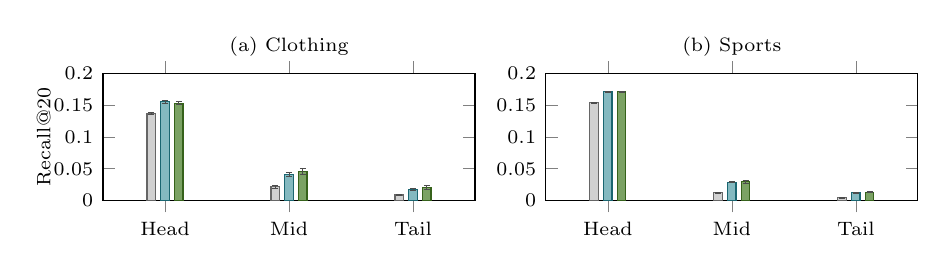
\begin{tikzpicture}
\begin{groupplot}[
  group style={group size=2 by 1, horizontal sep=9mm},
  width=0.52\columnwidth, height=3.2cm,
  ybar, /pgf/bar width=3.0pt,
  enlarge x limits=0.25,
  ymin=0, ymax=0.20,
  ytick={0,0.05,0.10,0.15,0.20},
  ylabel style={font=\scriptsize, yshift=-2mm},
  symbolic x coords={Head, Mid, Tail},
  xtick=data,
  xticklabel style={font=\scriptsize},
  yticklabel style={font=\scriptsize, /pgf/number format/fixed,
                    /pgf/number format/precision=2},
  title style={font=\scriptsize, yshift=-1.2mm},
  error bars/y dir=both,
  error bars/y explicit,
  error bars/error bar style={line width=0.3pt, black!70},
  error bars/error mark options={rotate=90, mark size=1.1pt,
                                 line width=0.3pt, black!70},
]
\nextgroupplot[title={(a) Clothing}, ylabel={Recall@20}]
\addplot+[fill=black!18, draw=black!60]
  plot [error bars/.cd, y dir=both, y explicit]
  coordinates {(Head,0.1365) +- (0,0.0018)
               (Mid,0.0221)  +- (0,0.0023)
               (Tail,0.0089) +- (0,0.0009)};
\addplot+[fill=accentteal!55, draw=accentteal!80!black]
  plot [error bars/.cd, y dir=both, y explicit]
  coordinates {(Head,0.1550) +- (0,0.0017)
               (Mid,0.0413)  +- (0,0.0026)
               (Tail,0.0176) +- (0,0.0009)};
\addplot+[fill=passgreen!70, draw=passgreen!80!black]
  plot [error bars/.cd, y dir=both, y explicit]
  coordinates {(Head,0.1527) +- (0,0.0023)
               (Mid,0.0452)  +- (0,0.0048)
               (Tail,0.0204) +- (0,0.0028)};
\nextgroupplot[title={(b) Sports}]
\addplot+[fill=black!18, draw=black!60]
  plot [error bars/.cd, y dir=both, y explicit]
  coordinates {(Head,0.1537) +- (0,0.0009)
               (Mid,0.0125)  +- (0,0.0006)
               (Tail,0.0045) +- (0,0.0006)};
\addplot+[fill=accentteal!55, draw=accentteal!80!black]
  plot [error bars/.cd, y dir=both, y explicit]
  coordinates {(Head,0.1712) +- (0,0.0007)
               (Mid,0.0288)  +- (0,0.0008)
               (Tail,0.0127) +- (0,0.0006)};
\addplot+[fill=passgreen!70, draw=passgreen!80!black]
  plot [error bars/.cd, y dir=both, y explicit]
  coordinates {(Head,0.1712) +- (0,0.0008)
               (Mid,0.0295)  +- (0,0.0021)
               (Tail,0.0132) +- (0,0.0006)};
\end{groupplot}
\end{tikzpicture}

\vspace{0.4mm}
{\scriptsize
\raisebox{0.4pt}{\tikz{\fill[black!18] (0,0) rectangle (1.7mm,1.7mm);\draw[black!60,line width=0.3pt] (0,0) rectangle (1.7mm,1.7mm);}}~MMHCL (5-seed)\quad
\raisebox{0.4pt}{\tikz{\fill[accentteal!55] (0,0) rectangle (1.7mm,1.7mm);\draw[accentteal!80!black,line width=0.3pt] (0,0) rectangle (1.7mm,1.7mm);}}~PACER (100~ep)\quad
\raisebox{0.4pt}{\tikz{\fill[passgreen!70] (0,0) rectangle (1.7mm,1.7mm);\draw[passgreen!80!black,line width=0.3pt] (0,0) rectangle (1.7mm,1.7mm);}}~PACER (250~ep)}
\caption{RQ3/RQ5 --- Recall@20 by popularity tercile, five-seed
mean~$\pm$~std from Table~\ref{tab:longtail}.
A common $y$-axis scale is held fixed so the two catalogues remain comparable.
\dvr lifts Mid/Tail on both at $100$~ep and reallocates further from Head
at $250$~ep; the effect is stronger on Sports. MMHCL bars use native
$d{=}64$; see Table~\ref{tab:longtail} for the capacity-matched control.}
\label{fig:tercile}
\end{figure}

\begin{table}[!htbp]
\caption{RQ3/RQ5 --- Recall@20 by item-popularity tercile (equal-sized
up to integer rounding: Clothing $7{,}678/7{,}678/7{,}677$; Sports
$6{,}119$ each). Five fixed seeds throughout. A1 is the \dvr
leave-one-out ablation ($\lambda_{\text{cl}}{=}0$);
$\Delta_{\text{DVR}}$ is the paired A0$-$A1 contrast.
Head refers to A0-vs.-A1 within the matched pipeline (statistically
flat), not to any cross-model comparison. Cross-model $\Delta\%$ rows
are quoted against the capacity-matched MMHCL$_{320}$ control; all
values are test-side. Boldface highlights the
Mid/Tail cells of the $\Delta_{\text{DVR}}$ row --- the primary
long-tail evidence.}
\label{tab:longtail}
\centering
\renewcommand{\arraystretch}{1.02}
\setlength{\tabcolsep}{2.5pt}
\resizebox{\columnwidth}{!}{%
\begin{tabular}{lcccc}
\toprule
\multicolumn{5}{l}{\textbf{Panel~A. Amazon Clothing}} \\
Model & R@20 (all) & R@20 (Head) & R@20 (Mid) & R@20 (Tail) \\
\midrule
MMHCL, native $d{=}64$ &
  $0.0874_{\pm 0.0007}$ &
  $0.1365_{\pm 0.0018}$ &
  $0.0221_{\pm 0.0023}$ &
  $0.0089_{\pm 0.0009}$ \\
MMHCL, capacity-matched $d{=}320$ &
  $0.0940_{\pm 0.0004}$ &
  $0.1404_{\pm 0.0024}$ &
  $0.0363_{\pm 0.0044}$ &
  $0.0169_{\pm 0.0014}$ \\
PACER-full, $100$-ep (A0) &
  $0.1039_{\pm 0.0008}$ &
  $0.1550_{\pm 0.0017}$ &
  $0.0413_{\pm 0.0026}$ &
  $0.0176_{\pm 0.0009}$ \\
A1 -- w/o \dvr, $100$-ep &
  $0.1028_{\pm 0.0006}$ &
  $0.1545_{\pm 0.0011}$ &
  $0.0389_{\pm 0.0027}$ &
  $0.0157_{\pm 0.0017}$ \\
$\Delta_{\text{DVR}}$ (A0$-$A1) &
  $+0.0011$ ($+1.1\%$) &
  $+0.0004$ ($+0.3\%$) &
  $\mathbf{+0.0024\;({+}6.1\%)}$ &
  $\mathbf{+0.0019\;({+}12.1\%)}$ \\
\midrule
PACER-full ($250$\,ep) &
  $0.1039_{\pm 0.0008}$ &
  $0.1527_{\pm 0.0023}$ &
  $0.0452_{\pm 0.0048}$ &
  $0.0204_{\pm 0.0028}$ \\
$\Delta\%$ ($250$\,ep) vs.\ MMHCL$_{320}$ &
  $+10.5\%$ &
  $+8.7\%$ &
  $+24.5\%$ &
  $+20.8\%$ \\
\midrule
\multicolumn{5}{l}{\textbf{Panel~B. Amazon Sports (Optuna-tuned)}} \\
Model & R@20 (all) & R@20 (Head) & R@20 (Mid) & R@20 (Tail) \\
\midrule
MMHCL, native $d{=}64$ &
  $0.1050_{\pm 0.0007}$ &
  $0.1537_{\pm 0.0009}$ &
  $0.0125_{\pm 0.0006}$ &
  $0.0045_{\pm 0.0006}$ \\
MMHCL, capacity-matched $d{=}320$ &
  $0.1128_{\pm 0.0006}$ &
  $0.1624_{\pm 0.0008}$ &
  $0.0202_{\pm 0.0007}$ &
  $0.0090_{\pm 0.0002}$ \\
PACER-full, $100$-ep (A0) &
  $0.1208_{\pm 0.0006}$ &
  $0.1712_{\pm 0.0007}$ &
  $0.0288_{\pm 0.0008}$ &
  $0.0127_{\pm 0.0006}$ \\
A1 -- w/o \dvr, $100$-ep &
  $0.1186_{\pm 0.0012}$ &
  $0.1711_{\pm 0.0014}$ &
  $0.0208_{\pm 0.0014}$ &
  $0.0077_{\pm 0.0008}$ \\
$\Delta_{\text{DVR}}$ (A0$-$A1) &
  $+0.0022$ ($+1.9\%$) &
  $+0.0002$ ($+0.1\%$) &
  $\mathbf{+0.0079\;({+}38.1\%)}$ &
  $\mathbf{+0.0050\;({+}65.3\%)}$ \\
\midrule
PACER-full ($250$\,ep) &
  $0.1209_{\pm 0.0005}$ &
  $0.1712_{\pm 0.0008}$ &
  $0.0295_{\pm 0.0021}$ &
  $0.0132_{\pm 0.0006}$ \\
$\Delta\%$ ($250$\,ep) vs.\ MMHCL$_{320}$ &
  $+7.2\%$ &
  $+5.4\%$ &
  $+45.7\%$ &
  $+46.5\%$ \\
\bottomrule
\end{tabular}%
}
\end{table}

% =====================================================================
\subsection{RQ4 --- Auxiliary Axes Factorial Audit}
\label{sec:factorial}
% =====================================================================

We audit a Data axis (RSFPGrowth source blend for the TAMER Interest
Tree~\cite{meng2025tamer}) and a Loss axis (Log$Q$-Laplace), with
\dvr enabled in all four cells (Table~\ref{tab:factorial}). Under
paired $t$, disabling both beats enabling both by $+0.049$~pp (B11
vs.\ B00, $p{=}0.040$, dir 5 of 5); each single-axis contrast is
non-significant (Data, B11 vs.\ B10, $p{=}0.074$; Loss, B11 vs.\ B01,
$p{=}0.82$). Neither axis adds measurable value once \dvr is present.

\begin{table}[!htbp]
\caption{RQ4 --- $2{\times}2$ factorial audit (Clothing, five seeds,
$100$-ep, R@20 $\times 100$). Rows: Log$Q$-Laplace; columns:
RSFPGrowth blend $\alpha$. \dvr is on and $\tau{=}0.30$ in all four
cells. Labels follow the internal run naming, where $1$ denotes the
disabled setting: B11 has both axes off (PACER's configuration;
Tables~\ref{tab:rq1}--\ref{tab:longtail} report an independent run of
it, indistinguishable at paired $p{=}0.52$), B00 both on.}
\label{tab:factorial}
\centering
\renewcommand{\arraystretch}{1.02}
\setlength{\tabcolsep}{4pt}
\begin{tabular}{lcc}
\toprule
Config & RSFP $\alpha{=}0.10$ & RSFP $\alpha{=}0$ \\
\midrule
Log$Q$ on  & B00: $10.358_{\pm 0.069}$ & B01: $10.400_{\pm 0.074}$ \\
Log$Q$ off & B10: $10.377_{\pm 0.058}$ &
  \textbf{B11: $\mathbf{10.407_{\pm 0.035}}$} \\
\bottomrule
\end{tabular}
\end{table}

% =====================================================================
\subsection{RQ5 --- Between-Dataset Replication (Amazon Sports)}
\label{sec:rq5}
% =====================================================================

We repeat RQ2 on Sports after an independent Optuna sweep
(Tables~\ref{tab:ablation}--\ref{tab:longtail},
Fig.~\ref{fig:tercile}b). In the matched ablation \dvr adds
$+38.1\%$ Mid and $+65.3\%$ Tail ($d_z{=}4.32/5.52$,
$p{<}10^{-3}$), with Head flat ($d_z{=}0.11$).
The cross-dataset gap is a \emph{steeper popularity gradient} (not
raw density): under MMHCL's native $d{=}64$ configuration the
Head{:}Mid{:}Tail R@20 ratio is
$12.3{:}1{:}0.36$ on Sports vs.\ $6.2{:}1{:}0.40$ on Clothing, so
neighbourhood averaging fails first on thin neighbourhoods, where
\dvr's SAV/IAV consensus supplies structure-aware signal --- hence the
${\approx}6{\times}$ larger Sports $\Delta_{\text{DVR}}$. The $250$-epoch schedule sharpens the
trade-off (Mid $+45.7\%$, Tail $+46.5\%$ vs.\ MMHCL$_{320}$, paired
$p{\le}3{\times}10^{-4}$, dir 5 of 5) at unchanged
overall Recall@20, mirroring Sec.~\ref{sec:rq3}.

% =====================================================================
\section{Conclusion}
% =====================================================================

PACER's finding is \emph{distributional}: a $d{+}2$-parameter
two-view denoiser (\dvr) reallocates capacity from Head to Mid/Tail
at nearly constant overall Recall@20. In the matched A0-vs.-A1
pipeline \dvr adds $+6.1\%$ Mid and $+12.1\%$ Tail on Clothing and
$+38.1\%$ Mid and $+65.3\%$ Tail on Sports, with Head flat on both
and overall Recall@20 statistically unchanged ($p{=}0.90$ at $250$
epochs). Against a capacity-matched MMHCL baseline at the same
embedding width, PACER lifts Clothing Recall@20 by $+10.48\%$ and
NDCG@20 by $+13.07\%$ ($+7.04\%$/$+8.56\%$ on Sports), with
$250$-epoch Mid/Tail gains of $+24.5\%$/$+20.8\%$, and a
$2{\times}2$ audit found neither auxiliary axis helpful.
Practically, \dvr offers marketplaces a way to buy catalogue coverage
without paying for it in aggregate accuracy.

\noindent\textbf{Limitations.} We evaluate on two Amazon catalogues
and a single backbone family. Our capacity control shows embedding
width alone explains much of the nominal cross-model margin, and depth
and protocol differences remain uncontrolled, so Table~\ref{tab:rq1}
is context rather than attribution. IAV's single shared
$g$ restricts compatibility to one rank-one latent direction;
multi-head or user-conditioned probes may be more expressive. Future work
composes \dvr with denoising-diffusion negative
sampling~\cite{nguyen2024diffusion} and tests transfer to non-MMHCL
backbones.

% =====================================================================
\bibliographystyle{IEEEtran}
\bibliography{references_v6}
% =====================================================================

\end{document}
